\section{Union-Find Disjoint Set (UFDS)}
\begin{frame}
  \begin{center}
    Hand-made Data Structures: The Union-Find Disjoint Set (UFDS)\\
    (CP4 2.4.2)
  \end{center}
\end{frame}


\subsection{Union-Find}
\begin{frame}
  \frametitle{Union-Find Disjoint Set (UFDS)}
  \framesubtitle{Motivating Problem}

  \begin{block}{Network Connections -- UVA793}
    We define a network with $n$ computers. Using the commands "c" and "q", we {\bf set} and {\bf test} the connection between the computers.
    \bigskip

    {\bf Input:} The number of computers $n$, and a sequence of commands:
    \begin{itemize}
    \item c i j -- Make computer $i$ and $j$ connected.
    \item q i j -- Ask if computer $i$ is connected to computer $j$. (yes/no)
    \end{itemize}

    \bigskip
    {\bf Output:} The number of queries (q) with answer "yes", and the number
    of queries with answer "no".
  \end{block}
\end{frame}

\begin{frame}
  \frametitle{Union-Find Disjoint Set (UFDS)}
  \framesubtitle{Motivating Problem -- Naive answer}

  \begin{block}{Neighborhood Graph}
    \begin{itemize}
    \item Initialize an $n\times n$ matrix with zeros.
    \item For every ``c i j'' input, $N_{i,j}$ and $N_{j,i}$ becomes 1.
    \item For every ``q i j'', we perform a breadth first search on the graph.
    \end{itemize}
  \end{block}


  \bigskip

  How good is this solution?
  \begin{itemize}
  \item Cost to insert a new connection: $O(1)$
  \item Cost to check if ``q i j'': $O(V+E)$
  \end{itemize}

  \bigskip We can do better!
\end{frame}

\begin{frame}
  \frametitle{Union-Find Disjoint Set}

  \begin{center}
    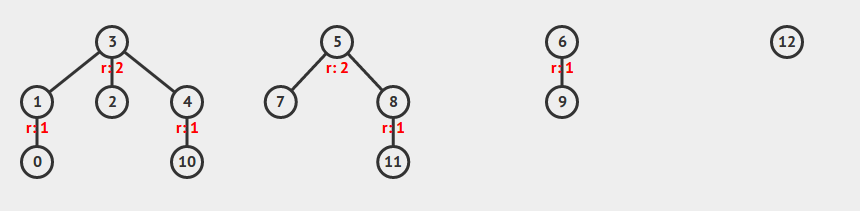
\includegraphics[width=.9\textwidth]{img/ufds1}
  \end{center}

  \begin{itemize}
  \item The UFDS keeps \structure{sets of items}, each is represented by a \structure{parent};
  \item When you join two sets \structure{You join their parents};
  \item When you test the parent of an item \structure{You flatten the tree};
  \item Test\_item and Join\_item are both O(1);\hfill \emph{(amortized)}
  \item Visualization: \url{https://visualgo.net/ja/ufds};
  \end{itemize}
\end{frame}

\begin{frame}[fragile]
  \frametitle{UFDS Implementation using Arrays}

  {\small
\begin{verbatim}
int p[MAX], r[MAX];
                             # which groups x belong to?
int find(int x) { return x == p[x] ? x : p[x]=find(p[x]); }

int join(int x, int y) {     # x and y are the same group
    x = find(x), y = find(y);
    if(x != y) {
        if(r[x] < r[y])     { p[x] = y; r[y] += r[x]; }
        else                { p[y] = x; r[x] += r[y]; }
        return 1;
    }
    return 0;
}
void init() { # Initialize each element as separate group
    for(int i = 0; i < MAX; i++)  { p[i] = i; r[i] = 1; }
}
\end{verbatim}
}

\end{frame}
